\documentclass{article}

\usepackage[T1]{fontenc}
\usepackage{natbib}
\usepackage{graphicx}
\usepackage[francais]{babel}
\usepackage[utf8]{inputenc}
\usepackage{fancyhdr}

\title{Rapport Projet Web : Bakaraoke}
\author{
  Cecconi Quentin
  \and
  Chatelet Leo
  \and
  Goyard Louis
  \and
  Sadler Alec
}
\date{May 2020}

\renewcommand*\contentsname{Sommaire}

\begin{document}

\pagestyle{fancy}
\fancyhf{}
\lhead{Projet Web 1A}
\rhead{Shinbakanim}
\rfoot{Page \thepage}
\maketitle
\newpage
\tableofcontents
\newpage

%Ici on input nos sections, comme les exemples ci dessous%
\section{introduction}
Ce rapport porte sur la créations et les fonctionnalitées du site Shinbakanim

\section{Structure du projet}
\subsection{Modèle Vue/Controlleur}
Pour l'apparence visuel du site nous avons adopté le modèle vue/controlleur. \\
Cela s'avère particulièrement utile pour l'affichage du header qui permet à l'utilisateur d'accéder à toutes les fonctionnalités du site, et ce quelque soit la page sur laquelle il se trouve actuellement.\\
Chaque page du site inclus donc la vue de ce header en entête, puis une vue de la page en question.
Par exemple la page login.php inclus la vue header.php ainsi que la vue de login.php (une autre page qui n'est pas dans public).\\
L'affichage des images de profil est aussi gérée par des vues et plus précisément par des fonctions php qui permettent d'afficher une image et de décider de ses dimensions ainsi que de sa forme en retournant une balise avec du CSS.\\
On retrouve dans le dossier \texttt{/public/Forms} les fichiers php qui s'occupe de la manipulation de la base de donnée côté serveur, avec par exemple \texttt{login.php} ou \texttt{addKara.php}.\newline
Les interfaces User, Lector, Playlist, et Kara se trouvent respectivement dans leur dossier respectifs dans le \texttt{/src}.


\subsection{Apparence visuelle}
Pour assurer qu'aucun style directement implémenté dans le html ne se fasse écraser par la feuille de style, l'utilisation de classe à été privilégié pour mieux contrôler les balises sur lesquelles le style s'applique. Une feuille de style, style.css, est commune à toutes les pages (car présente dans le head que l'on inclus systématiquement). Il est cependant possible d'intégrer d'autres feuilles de style pour des pages spécifiques.

\subsection{la base de donnée}
On rajoute plusieurs tables à la base de données pour pouvoir gérer les cosmétiques de chaque utilisateur et leur playlist, et la queue et la liste des lecteur du côté de lektor, voici le diagramme UML de la base de donnée du site:
\newline
\begin{figure}[h!]
\centering
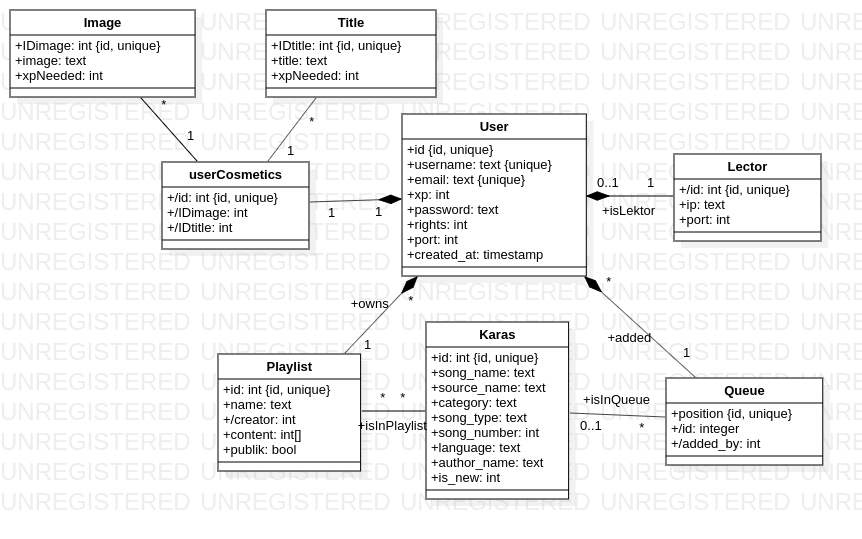
\includegraphics[scale=0.4]{UML.png}
\caption{diagramme UML de la base}
\label{fig:diagramme UML}
\end{figure}

\section{Sécurité}
    Un minimum de sécurité a été implanté pour éviter des attaques récurrentes comme un ddos ou des injections SQL :\newline
Chaque variable obtenue d'un formulaire via la méthode POST sera d'abord filtré avec la commande htmlspecialchars() pour éviter que des caractères spéciaux apparaissent. Ensuite, ces variables seront rentrées en paramètres dans les commandes SQL via la méthode bindParam du PDO.\newline
Lors d'une création, d'une connexion ou de la modification d'un compte, on vérifie bien que les champs remplis sont bien valides (email au bon format, pas d'espace dans le username), ainsi nous n'aurons pas de risque concernant l'utilisateur qui rentre une commande de type 'DROP TABLE'.\newline
Chaque formulaire aura avant tout une validation javaScript pour ne pas surcharger le serveur par de mauvaises requêtes.\newline\newline

Pour éviter que l'utilisateur ne "spam" les listes de lectures, on utilise le fichier "ddosPreventer.php" qui limite à 6 le nombre de requêtes toutes les 30 secondes. On utilise aussi ce fichier au moment du login ou de l'inscription. 


\section{Utilisateurs}

Lorsque qu'un client arrive pour la première fois sur le site, il n'aura pas accès aux différents services du site. Il devra d'abord se créer un compte sur la page registration.php, ici il entrera ses 
identifiants comme son adresse email, son nom d'utilisateur, et son mot de passe.\newline
Il est à noter qu'un utilisateur ne peut pas avoir d'espace dans son nom, ce qui permet d'avoir une sécurité supplémentaire contre les injections SQL.\newline
Après vérification javascript d'un formulaire, on récupère et envoie ces informations à la page addUser.php qui va les insérer dans la table "user", le mot de passe sera hashé pour éviter toute tentative de vol de mot de passe. Tout transfert d'information se fera via la méthode POST, afin de transférer les données de manière sécurisée.
\newline

Ces informations peuvent être  ultérieurement modifiées sur la page modifyUser.php, qui enverra les modifications à modifyUserAccount.php.\newline

Une fois qu'un utilisateur s'est créé un compte, il peut se connecter via login.php. Si il le fait, on démarre une session et on initialise les attributs de la variable de session, c'est avec ces attributs qu'on déterminera si la session est ouverte, et qu'on affichera les cosmétiques de l'utilisateur.

\subsection{Personnaliser son compte}

Aussi, après ajout d'un utilisateur dans "user", on insère une nouvelle ligne dans la table "UserCosmetics", cette table permet de savoir quel sont les cosmétiques choisis par l'utilisateur.  
Chaque utilisateur aura accès à une liste d'images de profil et de titres qu'il pourra sélectionner pour customiser son profil. Ces cosmétiques sont contenus dans les tables "Image" et "Titles".
\newline
Ces images ne sont pas toutes disponibles dès le départ. En effet chaque utilisateur possède des points d'expérience, initialisés à 0 à la création du compte, qui peuvent être gagné lorsqu'un kara est rajouté à une playlist. Les images se débloquent au fur et à mesure que l'utilisateur passe du temps sur le site. Sur ChangePP.php seules les images et titres dont xpNeeded<SESSION['xp'] sont affichés.\newline
Pour pouvoir modifier son compte, l'utilisateur doit se rendre sur changePP.php, pour modifier son image de profil et/ou son titre. Un formulaire envoie les informations à modifyUserCosmetics.php. L'utilisateur a le choix entre les différentes images contenues dans la table "Images" et les différents titres dans "Titles". \newline

\subsection{Les playlists}

Un utilisateur peut créer ses propres playlists de karas disponibles dans la table "Karas".
D'ici il pourra ajouter cette playlist dans la Queue du lecteur, ou simplement retrouver les karas qu'il préfère afin de les ajouter.
Toutes ces informations sont contenues dans la table Playlist, et les utilisateurs peuvent regarder les playlists des autres utilisateurs si elles sont paramétrées comme étant publique.\newline
Une playlist ne peut cependant être éditée que par son créateur.\newline

\subsection{Droits des utilisateurs}
Lorsqu'un utilisateur se register dans la base de donnée, on lui attribut un droit 0. Les différents droits sont définis par des entiers:
\begin{itemize}
	\item 0 pour un utilisateur lambda
	\item 1 pour un admistrateur
	\item 2 pour un super-administrateur
\end{itemize}
Un utilisateur a la possibilité de révoquer ou d'augmenter les droits d'un utilisateur ayant un droit inférieur. Ceci se fait sur la page admin.php, page seulement accessible par les admins. C'est en vérifiant les attributs de la session actuelle (SESSION) qu'on détermine si l'utilisateur est bien un admin.

\section{Queue et Lektor}
\subsection{Queue}

La queue, qui est une "playlist courante", est une table de karaokes. Ses deux principaux attributs sont la position et l'id du karaoke. Elle représente donc une liste ordonnée de karaokes à être lus.

Elle possède aussi un attribut \texttt{added\_by}, qui permet de savoir quel utilisateur à ajouter chaque karaoke de la queue.

La queue est donc unique et n'importe quel utilisateur peut ajouter des karaokes à celle-ci.
L'ajout se fait avec une requête \texttt{POST} à la page \texttt{/Forms/addKara.php}, en fournissant l'id du karaoke que l'on veut rajouter. Cette page va effectuer la requête, en s'assurant tout d'abord que l'utilisateur est connecté, et, si il n'est pas un administrateur, qu'il n'ajoute pas trop de karaokes en un temps restreint.
Afin de pouvoir trouver facilement les karaokes voulus dans la queue, la liste de karaokes entière est chargé sur la page html et affichée sous forme de liste de formulaire. Une barre de recherche permet de rentrer des mot-clés, ce qui va executer une fonction javascript qui va cacher les karaokes qui ne correspondent pas. Cela permet aux utilisateurs de faire des recherches rapides et de ne pas surcharger le serveur de requêtes (la table \texttt{kara} n'ayant pas vocation à changer durant une
session).
Seul les administrateurs peuvent supprimer des karaokes de la queue à travers une requête \texttt{POST} vérifiant les droits nécessaires à travers la variable \texttt{\$\_SESSION{\lbrack'rights'\rbrack}} 
L'état actuel de la queue peut être récupérée grâce à la page \texttt{/Forms/getQueue.php} à l'aide d'une requête \texttt{GET}.

\subsection{Lector}

Lektor est un logiciel de lecture de karaoke. Il fonctionne avec une architecture client-serveur permettant de faire tourner un daemon (lektord) sur son ordinateur, auquel on peut envoyer des commandes à l'aide d'un client (lkt) ou bien tout simplement à l'aide d'une socket ou de netcat. Lektord va ensuite, en fonction des commandes qu'il reçoit, lire les karaokes voulu sur le système où il tourne. Il respecte le protocole MPC, bien qu'étant encore en développement (par des élèves de
l'ENSIIE).\newline
Pour pouvoir faire fonctionner lektor sur son pc, une explication se trouve à la racine du projet dans le readMe.\newline

C'est ce logiciel qu'utilise notre site pour lire des karaokes : chaque utilisateur peut, si il le souhaite et qu'il possède sur son ordinateur personnel la base de données de karaokes ainsi que lektord, s'ajouter sur le site en tant que lecteur. Il faut pour celà avoir l'adresse IP du client, qui est récupéra à l'aide de \texttt{\$\_SERVER\lbrack'HTTP\_CLIENT\_IP'\rbrack}, \texttt{\$\_SERVER\lbrack'HTTP\_X\_FORWARDED\_FOR'\rbrack} ou bien \texttt{\$\_SERVER\lbrack'REMOTE\_ADDR'\rbrack}.
L'utilisateur doit aussi signaler le port sur lequel son lektord écoute (si non renseigné, la valeur par défaut est le port 6600, qui est la valeur par défaut de lektord).
Ces informations sont stockés dans la base de données.
Une information plus "volatile" est stockée dans la variable \texttt{\$\_USER\lbrack'is\_lector'\rbrack}, qui permet de savoir si un utilisateur est un lecteur sans faire appel à la base de donnée.

Ensuite, à chaque changement impactant la queue (ajout ou retrait de karaoke), le serveur va récuperer la liste des lecteurs dans la base de donnée, puis envoyer les commandes correspondantes aux lecteurs à l'aide de sockets php.
L'implémentation actuelle du site envoie juste les sockets une par une aux différents lektor, avec un timeout de 4 secondes afin d'éviter qu'un lecteur injoignable ne bloque totalement le site. L'implémentation actuelle n'est donc pas vraiment optimale car l'information pourrait prendre un certain temps à atteindre les derniers lecteurs si les lecteurs précedents prennent du temps à accepter la connection. Pendant le développement, une version avec des forks php générés à l'aide de
\texttt{pcntl\_fork()} a été développé. Cependant, les processus fils ne s'arrêtait pas quand il le fallait, ce qui posait des problèmes de processus ne s'arrêtant jamais, et ce même en ayant un \texttt{exit} dans chaque processus enfants et en implémentant une boule de \texttt{pcntl_waitpid} dans le processus parent afin d'attendre que tout les processus enfants soient terminés pour quitter.

\section{Conclusion}
Notre site Bakaraoké a donc rempli les objectifs fixés par le projet, que ce soit la gestion d'utilisateurs
avec en plus un ajout de personnalisation, l'utilisation de scripts pour protéger le site ou encore la gestion
de tables permettant de gérer les karaokés de la base de donnée et la création de playlists.\newline
\newline
Nous pensons que l'amélioration du site se fera à partir de maintenant sur l'approfondissement de la personnalisation des comptes
et des playlists, en permettant de créer des playlists collaboratives par la modification de la table pour rajouter un champ collaborateur,
ou l'ajout d'une fonctionnalité de lecture directe sur le site en ajoutant le lecteur de vidéos sur le site.

\end{document}
